\documentclass[]{scrreprt}
\usepackage{amsmath,amsfonts,graphicx}

\newcommand{\uo}{\mbox{UO\textsubscript{2}}\xspace}

\setcounter{secnumdepth}{3}


\begin{document}


\title{A comparison with Rehbinder's THM solution}
\author{CSIRO}
\maketitle

\tableofcontents

\chapter{Rehbinder's THM solution}

\section{Introduction}

Rehbinder\footnote{G Rehbinder (1995) ``Analytical solutions of
  stationary coupled thermo-hydro-mechanical solutions'' Int J Rock
  Mech Min Sci and Geomech Abstr 32, 453--463} derives analytical
solutions of cylindrically-symmetric and spherically-symmetric THM
problems in certain limits.  The solution is a steady-state THM solution
of a pressurised and
heated cavity of radius $r_{\mathrm{cavity}}$ in a finite domain of
radius $r_{\mathrm{outer}}$.  In the cylindrically-symmetric case the
cavity is a cylinder of radius $r_{\mathrm{cavity}}$ and the domain is
a cylinder of radius $r_{\mathrm{outer}}>r_{\mathrm{cavity}}$.  In
this document only the cylindrically-symmetric situation is explored.
The cylindrical coordinates are denoted by $(r, \phi, z)$.

\section{Initial and boundary conditions}

The initial conditions are zero porepressure, $P_{f}(t=0) = 0$;
zero temperature, $T(t=0) = 0$; and zero displacement $u(t=0)=0$.

The boundary conditions are at the cavity wall are
\begin{eqnarray}
P_{f}(r_{\mathrm{cavity}}) & = & P_{0} \ , \nonumber \\
T(r_{\mathrm{cavity}}) & = & T_{0} \ , \nonumber \\
\sigma_{rr}^{\mathrm{eff}}(r_{\mathrm{cavity}}) & = & 0 \ .
\end{eqnarray}
The latter condition implies the total radial stress is $-P_{0}$ at the
cavity wall, corresponding to the fluid in the cavity pushing on the
cavity wall.  The boundary conditions at the outer radius are
\begin{eqnarray}
P_{f}(r_{\mathrm{outer}}) & = & 0 \ , \nonumber \\
T(r_{\mathrm{outer}}) & = & 0 \ ,
\end{eqnarray}
and either $\sigma_{rr}^{\mathrm{eff}}(r_{\mathrm{outer}}) = 0$ or $u(r_{\mathrm{outer}})
= 0$.  In this document the former is called the ``free outer''
boundary condition, while the latter is called the ``fixed outer''
boundary condition.

\section{Simplifying assumptions}

In order to
derive the solution, Rehbinder makes various simplifications.
Translated to the language of the other PorousFlow documents these are
as follows.
\begin{enumerate}
\item There is no gravity.
\item All quantities depend only on the radial coordinate, $r$, and
  not the angular coordinate $\phi$ or the axial coordinate $z$.
\item Plane-strain is assumed, so $\epsilon_{zz}=0$.
\item There is only one fully-saturated fluid phase that contains one component.
\item The fluid relative permeability is unity.
\item The fluid density is constant.  In the numerical simulation
  below, the density is assumed to obey $\rho =
  \rho_{0}e^{P_{f}/K_{f}}$, with $\rho_{0}=1000$\,kg.m$^{-3}$, and
  $K_{f}=10^{3}$\,GPa.
\item The fluid dynamic viscosity is constant.  In the numerical simulation
  below, the dynamic viscosity is $\nu=10^{-3}$\,Pa.s.
\item The Biot coefficient is unity $\alpha_{B}=1$.
\item The fluid internal energy is assumed to be linear in the
  temperature.  In the numerical simulation below, $\mathcal{E}=CT$
  where $C=1000$\,J.kg$^{-1}$.K$^{-1}$.
\item The fluid enthalpy is assumed to be equal to the fluid internal energy.
\item The velocity of the solid skeleton is zero: ${\mathbf v}_{s} =
  0$.  To model this using PorousFlow, the ``{\tt
    VolumetricExpansion}'' Kernels are not included.
\item The rock-matrix density is constant. In the numerical simulation
  below, the value $\rho_{R} =
  2500$\,kg.m$^{3}$ is chosen.
\item The rock-matrix specific heat capacity is constant.  In the
  numerical simulation below, the value
  $C_{R} = 1000$.J.kg$^{-1}$.K$^{-1}$ is chosen.
\item The rock deforms elastically (so there is no plastic heating).  In the numerical simulation
  below, the Young's modulus is $E=10$\,GPa and the Poisson's ratio is $\nu
  = 0.2$.
\item The porosity is constant.  In the simulation below $\phi=0.1$ is
  chosen.
\item The permeability is constant.  In the simulation below
  $k=10^{-12}$\,m$^{2}$ is chosen.
\item The thermal conductivity of the rock-fluid system is constant.
  In the simulation below $\lambda =
  10^{6}$\,J.s$^{-1}$.m$^{-1}$.K$^{-1}$ is chosen.
\item Steady-state heat flow, fluid-flow and mechanical deformation
  has been reached (Rehbinder equation (41)).  Using the aove
  assumptions, this is true if
  $t>\rho_{s}c_{s}r_{\mathrm{cavity}}/\lambda = r_{\mathrm{cavity}}$
  (the left-hand-side is measured in seconds, the right-hand-side in metres).  In the simulation
  below, steady-state is achieved by not including any time-derivative
  Kernels.
\item The liquid flow is quasi-stationary, in the sense that the
  diffusion of heat is much slower than the diffusion of pore pressure
  (Rehbinder equation (32)).  Using the above assumptions this may be
  written as $\phi\lambda\mu/K_{f} \ll \rho_{s}c_{s}k$ where $\lambda$
  is the thermal conductivity of the rock-fluid system, and
  $\rho_{s}c_{s} = (1-\phi)\rho_{R}C_{R} + \phi\rho C =
  2.35$\,MJ.K$^{-1}$.m$^{-3}$.  Using the above values, this condition reads
  $10^{6} \ll 2.35\times 10^{10}$ which is clearly satisfied.
\item The liquid flow is quasi-stationary, in the sense that a
  pressure change in the cavity is transmitted instantaneously through
  the pores to the outer boundary (Rehbinder equation (33)).  Using
  the above assumptions this may be written as $r_{\mathrm{outer}} -
  r_{\mathrm{cavity}} \ll \sqrt{k K_{f}/(\phi\nu)} = 100$\,m.  In the
  simulation below, $r_{\mathrm{cavity}}=0.1$\,m and
  $r_{\mathrm{outer}}=1$\,m are chosen.
\item The heat is mainly conducted through the matrix, and a
  negligible part is convected with the flux.  This is true if the
  Peclet number is very small (Rehbinder equation (35))
\begin{equation}
\mathrm{Pe} = \frac{\rho c \alpha_{T} T_{0} E
  k}{\mu\lambda(1-\nu)} \ll 1 \ .
\end{equation}
(Rehbinder writes this in terms of a reference temperature,
$T_{\mathrm{ref}}$, which is chosen here to be $T_{0}$.)  Using the
above values this is $\mathrm{Pe} = 1.25\times 10^{-5}\alpha_{T} T_{0} \ll 1$.
In the simulation below, $\alpha_{T} = 10^{-6}$\,K$^{-1}$ and $T_{0}=1000$\,K are chosen, yielding
$\mathrm{Re} = 0.0125$.
\end{enumerate}
Rehbinder's derives the solution of this THM problem as an expansion
in the Peclet number.  I shall not write the solution here as it is
fairly lengthy.  The paper contains a few minor typos and they are
corrected in the accompanying {\tt thm\_rehbinder.py} script.

\chapter{Comparison with PorousFlow}

The PorousFlow module is designed to simulate THM problems.  The
output compares favourably with Rehbinder's analytical solution, as
demonstrated in the figures below.

\begin{figure}[htb]
\centering
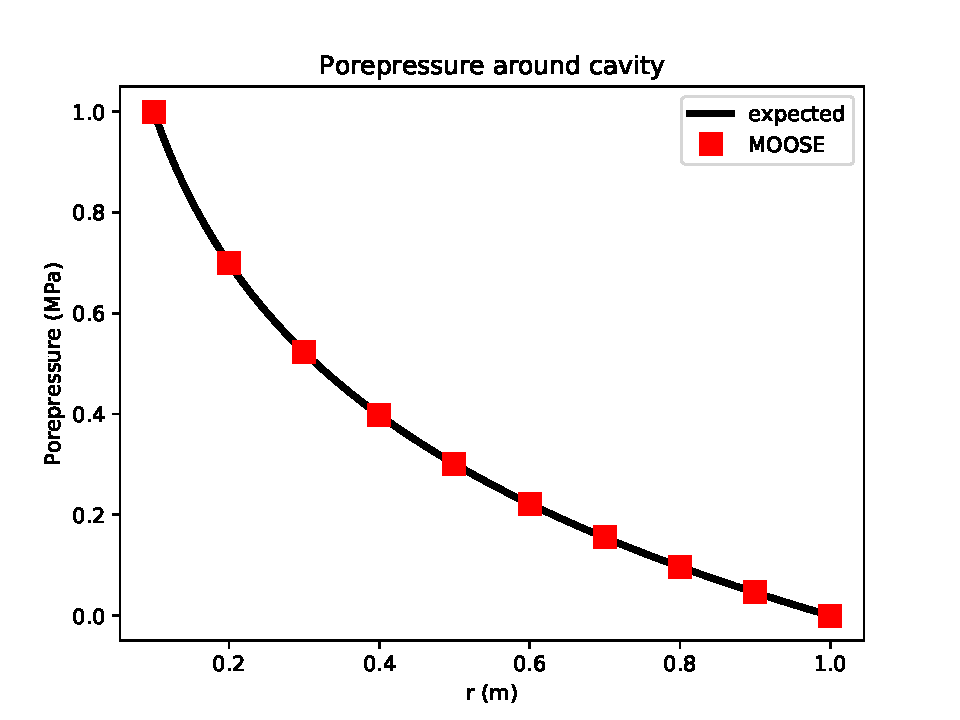
\includegraphics[width=15cm]{porepressure_fig.pdf}
\caption{Comparison between the MOOSE result (squares) and the
  analytic expression derived by Rehbinder for the porepressure.}
\label{porepressure_fig.fig}
\end{figure}

\begin{figure}[htb]
\centering
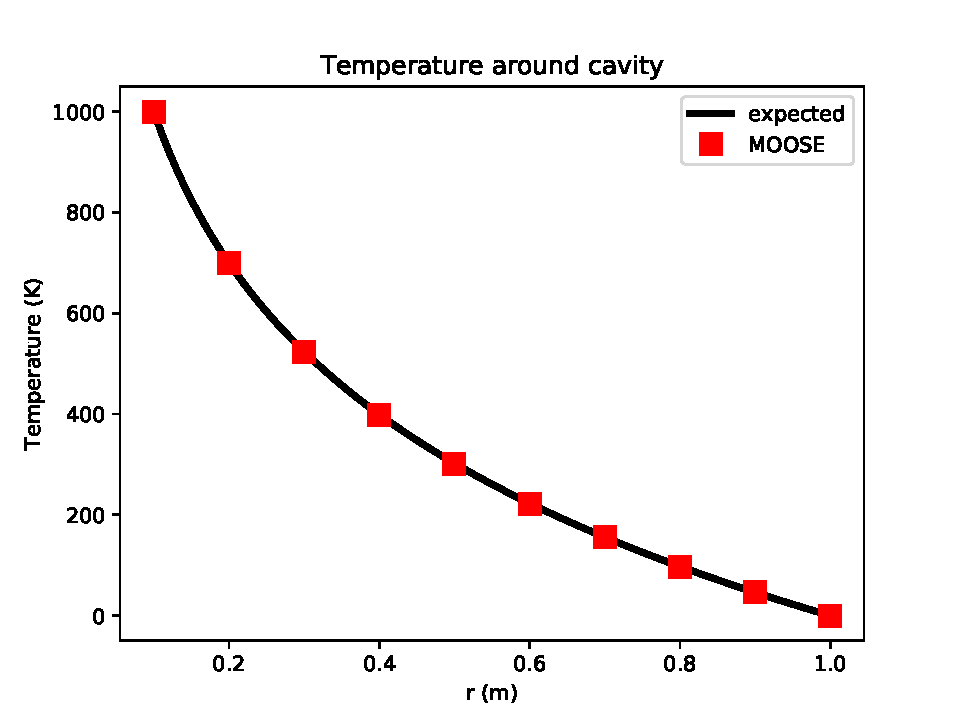
\includegraphics[width=15cm]{temperature_fig.pdf}
\caption{Comparison between the MOOSE result (squares) and the
  analytic expression derived by Rehbinder for the temperature.}
\label{temperature_fig.fig}
\end{figure}

\begin{figure}[htb]
\centering
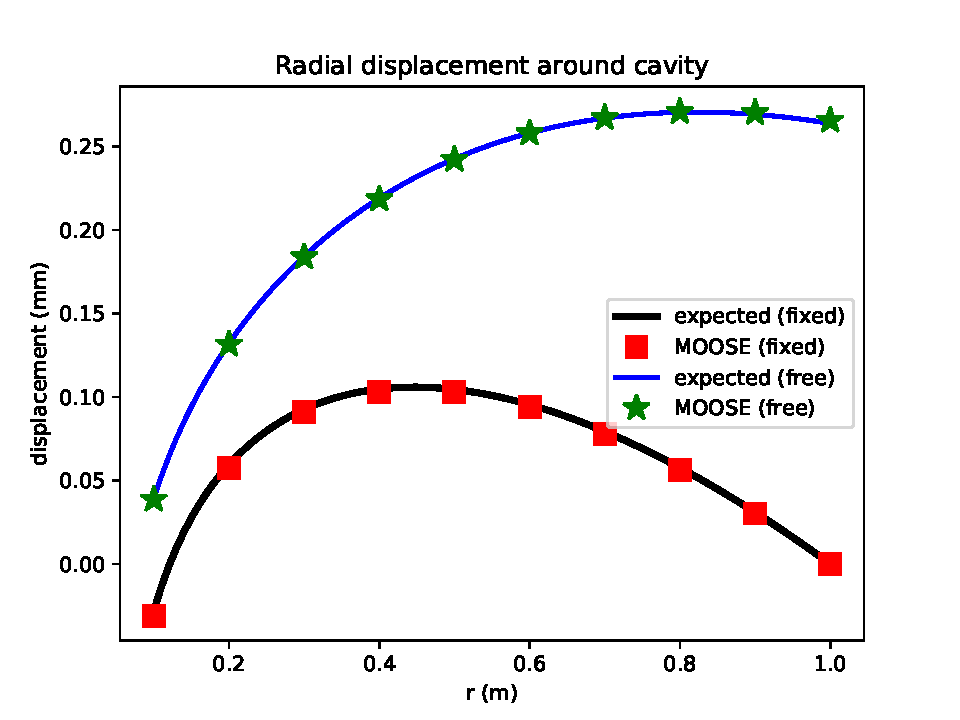
\includegraphics[width=15cm]{displacement_fig.pdf}
\caption{Comparison between the MOOSE results and the
  analytic expressions derived by Rehbinder for the radial
  displacement.  Both the fixed and free outer boundary conditions are
  shown.}
\label{displacement_fig.fig}
\end{figure}




\end{document}
